\section{Organic Chemistry}

\begin{multicols}{2}


\section*{Introduction to Organic \hfill \\ Chemistry}
% Fractional distillation of crude oil, cracking


%\subsection{Petroleum Jelly Glow}
%
%%\begin{center}
%%\includegraphics[width=0.4\textwidth]{./img/.png}
%%\end{center}
%
%\begin{description*}
%%\item[Subtopic:]{}
%\item[Materials:]{Petroleum jelly, black light}
%%\item[Setup:]{}
%\item[Procedure:]{Let the students put some petroleum jelly on their hands and then have them walk over to the black light. }
%%\item[Hazards:]{}
%%\item[Questions:]{}
%\item[Observations:]{hands will glow slightly purple.}
%\item[Theory:]{Petroleum jelly consists of long hydrocarbon chains that are one of the last products of crude oil distillation. Its molecular mass is very high and it has some conjugation in its structure. For reasons similar to those of quinine, these conjugated systems absorb UV light and fluoresce a purple light.}
%%\item[Applications:]{}
%%\item[Notes:]{}
%\end{description*}

\subsection[Showing the Presence of Carbon in Sugar]{Showing the Presence of \hfill \\ Carbon in Sugar}

%\begin{center}
%\includegraphics[width=0.4\textwidth]{./img/.png}
%\end{center}

\begin{description*}
%\item[Subtopic:]{}
\item[Materials:]{Metal spoon, sugar, candle}
%\item[Setup:]{}
\item[Procedure:]{Place the spoon above the flame of the candle.}
\item[Hazards:]{Be sure to use caution when using the flame as the spoon can get hot.}
%\item[Questions:]{}
\item[Observations:]{As the cap heats up it will heat the sugar. Heating the sugar will partially burn it before turning completely to carbon and carbon dioxide. This partial combustion is visible - as the sugar burns it turns brown and then black.}
\item[Theory:]{As sugar burns in air, it partially combusts, leaving behind carbon solid and other carbon compounds before changing into carbon dioxide. These carbon compounds have a brown color and the carbon solid compounds have a black color. As the sugar heats, it will combust until having a brown color, then to a black color. This black substance is solid carbon.}
\item[Applications:]{This is the same color as charcoal, which is another example of solid carbon. The browning of the sugar is called caramalization. As the sugar breaks down into smaller and different saccarides, they bring a very delicious taste. This is the process that is used very much in making different candies, especially toffees, brittles, and caramels. In fact, this is how many candies get their brown or dark color.}
%\item[Notes:]{}
\end{description*}

\subsection{Converting Soaps into Lipids or Fats}

%\begin{center}
%\includegraphics[width=0.4\textwidth]{./img/.png}
%\end{center}

\begin{description*}
%\item[Subtopic:]{}
\item[Materials:]{Powdered soap, battery acid, water, jam jar}
%\item[Setup:]{}
\item[Procedure:]{Take half of a spoon of powdered soap and dilute it to about 50 mL in a jam jar. Add about 2 mL of battery acid.}
\item[Hazards:]{Handle battery acid with care.}
%\item[Questions:]{}
\item[Observations:]{Bubbles of oil will form on the surface of the water.}
\item[Theory:]{Soaps are actually long chains of hydrocarbons with a protonated carboxylic acid group on the end. This protonated group allows soaps to cause oil and water to mix: it is both hydrophobic on one end and hydrophilic on the other. One end can dissolve in water while the other ends dissolves in the oil layer. This allows soap to be soluble in both water and oil solutions.}
\item[Applications:]{This is why soaps are used to clean off grease, oil, and other organic solvents. The organic solvents are hydrophobic and the soap can dissolve them.}
%\item[Notes:]{}
\end{description*}

\subsection{Cracking Household Oil}

\begin{center}
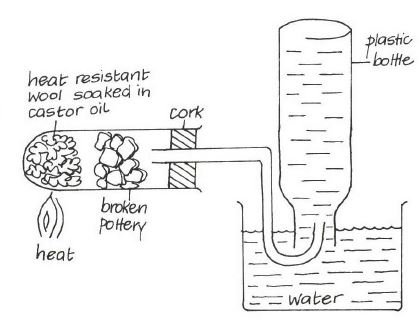
\includegraphics[width=0.45\textwidth]{./img/vso/cracking.jpg}
\end{center}

\begin{description*}
%\item[Subtopic:]{}
\item[Materials:]{Test tube/syringe, steel wool, two burners, oil, bottle, water}
\item[Setup:]{Take a narrow a test tube and place it at an angle. At the bottom, place some normal household oil. At the top, stuff in some steel wool so it does not move. Seal the tube with cork or a rubber stopper.}
\item[Procedure:]{Heat the steel wool until very hot. Then place a second burner under the oil so both the oil and the wool are being heated. After a minute or two, take a flame to the end of the tube.}
\item[Hazards:]{Handle flame with caution and be aware that gases produced are flammable.}
%\item[Questions:]{}
\item[Observations:]{The gases escaping the tube can sustain a flame.}
\item[Theory:]{\emph{Cracking} is a process where long hydrocarbon chains are heated so they are broken into smaller chains of molecules. Household oil is a triglyceride: a compound that has a glycerin backbone that has 3 long hydrocarbon arms. These long hydrocarbons range between 15 and 30 carbons long. These hydrocarbon arms can be broken easily by heating them in the presence of a catalyst, iron wool in this case. As they break down into smaller hydrocarbons, they become more volatile and combust easily. The long hydrocarbons will break down into hydrocarbon chains of 3 to 8 carbons. These will burn in air supporting a flame at the end of the tube.}
%\item[Applications:]{}
%\item[Notes:]{}
\end{description*}

\subsection{Petroleum Products}

%\begin{center}
%\includegraphics[width=0.4\textwidth]{./img/.png}
%\end{center}

\begin{description*}
%\item[Subtopic:]{}
\item[Materials:]{syringe with needle, 3 jam jars, as many as possible of: petrol, diesel, car lubricants, greases, petroleum jelly, kerosene, asphalt, tar, butane from a lighter}
\item[Setup:]{Place some petrol, kerosene, diesel, and any other petroleum product in different jam jars. For butane use a syringe to remove the butane from a lighter. There is usually a small hole where a needle can be inserted to add more butane gas. }
\item[Procedure:]{Compare the different properties of each of these compounds.}
\item[Hazards:]{Many petroleum products are quite flammable. Additionally the butane of a lighter is under pressure.}
\item[Questions:]{How do the density, viscosity, volatility, and flammability of the petroleum products compare and contrast?}
%\item[Observations:]{}
\item[Theory:]{We use many petroleum products every day. Crude oil is a black thick mixture of different hydrocarbons. To get different petroleum products, the crude oil is cracked and distilled to separate compounds depending on the number of carbon atoms. Butane is an early distillate since it has 4 carbons it distills easily. Petrol is an 8 carbon distillate. Kerosene has 12 to 15 carbons. Diesel has 15 to 25 carbons. Petroleum jelly is not a small hydrocarbon, but rather very long chains of varying length that does not distill easily. It is one of the last products from distilling crude oil.}
%\item[Applications:]{}
\item[Notes:]{If you want to make some mock crude oil to show students, mix road tar with kerosene until you have a viscous liquid.}
\end{description*}

\subsection{Preparation of Soap}

%\begin{center}
%\includegraphics[width=0.4\textwidth]{./img/.png}
%\end{center}

\begin{description*}
%\item[Subtopic:]{}
\item[Materials:]{Sunflower oil, caustic soda (sodium hydroxide), distilled water, salt, bottle, filter papers, \nameref{sec:heatsources}, beaker}
\item[Setup:]{Prepare a 1 M solution of sodium hydroxide and a concentrated salt water solution.}
\item[Procedure:]{Put about 25 mL of sunflower oil into an empty jar or bottle. Add about 100 mL of 1 M sodium hydroxide solution. Light the heat source and heat the mixture gently for 30 minutes so that the content mixes. Continue heating and stirring while adding distilled water from time to time until no more solids separate out. Allow the mixture to cool and then add brine (concentrated NaCl solution). Stir the mixture continuously for 5 minutes. Pour the solution into a fresh beaker and allow it to settle. The solution should solidify. Use a small piece of the solid soap to clean an oily piece of cloth.}
\item[Hazards:]{Sodium hydroxide (caustic soda) is corrosive to the skin and even in a dilute solution can blind. Avoid contact with skin and eyes. Neutralize spills with citric acid solution.}
\item[Questions:]{What is the chemical formula for soap formation? How could you prepare soap at home?}
%\item[Observations:]{}
\item[Theory:]{The soap is produced when sodium salt of fatty acid is produced from the reaction of vegetable oil with caustic soda. The soap cleans an oily piece of cloth.}
\item[Applications:]{The soap produced is sodium salt of fatty acid and is similar to the ordinary soap we buy in the market/shops.}
%\item[Notes:]{}
\end{description*}

\subsection{Acting Out Polymerisation}

\begin{center}
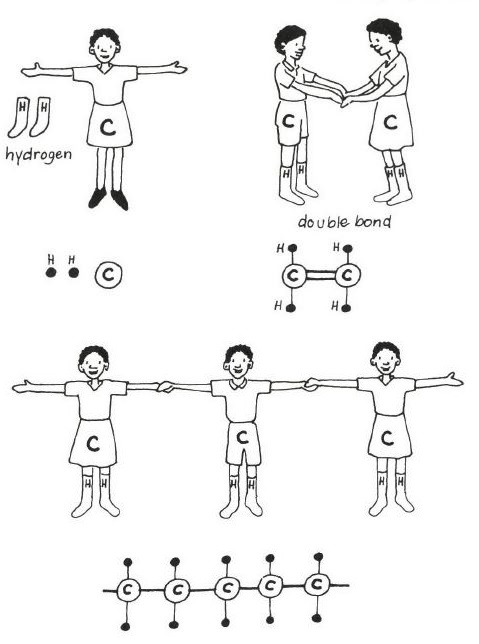
\includegraphics[width=0.49\textwidth]{./img/vso/polymerisation.jpg}
\end{center}

\begin{description*}
%\item[Subtopic:]{}
\item[Materials:]{Socks, students}
%\item[Setup:]{}
\item[Procedure:]{Students act out polymerisation of molecules by having a shirt or skirt represent carbon atoms and socks representing hydrogen atoms. Arms represent single or double bonds.}
%\item[Hazards:]{}
%\item[Questions:]{}
%\item[Observations:]{}
\item[Theory:]{The small molecule is ethene which polymerises to poly(ethene) - often called polythene.}
%\item[Applications:]{}
%\item[Notes:]{}
\end{description*}

\columnbreak

\subsection[Organic Chemistry Naming Game]{Organic Chemistry Naming \hfill \\ Game}

%\begin{center}
%\includegraphics[width=0.4\textwidth]{./img/.png}
%\end{center}

\begin{description*}
%\item[Subtopic:]{}
\item[Materials:]{Cardboard/styrofoam/any material which a toothpick can stick in, toothpicks, markers, deck of cards}
\item[Setup:]{Cut cardboard into small equal size pieces (at least 50) and label roughly a third of them ``C'', a few with ``O'', and the rest with ``H''. Write out on a piece of paper:\\

Diamond (``Kisu'') - Alkane\\
Spade (``Jembe'') - Alkene\\
Heart (``Moyo'') - Alkyne\\
Club (``Maua'') - Carboxylic Acid/Alcohol\\

K - Propyl Substituent\\
Q - Ethyl Substituent\\
J - Methyl Substituent \\

A - 1 Carbon atom\\
2 - 2 Carbon atoms\\
3 - 3 Carbon atoms\\
4 - 4 Carbon atoms\\
5 - 5 Carbon atoms\\
6 - 6 Carbon atom\\
7 - 7 Carbon atoms\\
8 - 8 Carbon atoms\\
9 - 9 Carbon atoms\\
10 - 10 Carbon atoms\\}
\item[Procedure:]{Draw a card from the deck and create a model of the organic molecule using the cardboard (Carbon, Hydrogen, and Oxygen atoms) and toothpicks (bonds) based on the card they receive. For example, a 3 of hearts would require the student to construct a three carbon alkyne molecule (propyne). \\

If a face card is drawn the student would draw another card and use the face card as a \emph{substituent} to add on to the molecule. (Ex: A player draws a queen and then takes another card which turns out to be a 7 of spades. The student must make a model of a 7 carbon alkene molecule (heptene) and add a ethyl substituent (due to the queen). In all cases the student must name the compound - here ethylheptene.) Points can be attributed to the complexity of molecules created and competitions can be made.}
%\item[Hazards:]{}
%\item[Questions:]{}
%\item[Observations:]{}
%\item[Theory:]{}
\item[Applications:]{Being able to understand the name and structure of organic chemicals is an important part of organic chemistry, and this game allows students to practice constructing structures and names for all the types of organic molecules that are learned in the O-level syllabus.}
%\item[Notes:]{}
\end{description*}

\columnbreak

%==================================================================================================%

\section*{Hydrocarbons}


\subsection{Alkanes}

%\begin{center}
%\includegraphics[width=0.4\textwidth]{./img/.png}
%\end{center}

\begin{description*}
%\item[Subtopic:]{}
\item[Materials:]{Butane lighter, petrol, kerosene, Vaseline, candle wax, pin/syringe needle.}
\item[Setup:]{Place each of the items (butane lighter, petrol, kerosene, Vaseline, and candle wax) on a desk in this order. (Use the needle to press the release valve on the underside of the butane lighter.) Write approximate chemical formulas for each compound. Butane is \ce C$_4$H$_{10}$; petrol is \ce C$_8$H$_{18}$, kerosene is about \ce C$_{12}$H$_{26}$, Vaseline is about \ce C$_{20}$H$_{42}$, and wax is about\ce C$_{25}$H$_{52}$. Note that these are only approximate formulas, especially for the larger molecules.}
\item[Procedure:]{Observe the visible properties of each alkane sample. Comment on the states of matter of each. Rank them from smallest molecules to largest. Note the correlation between molecule size and state of matter.}
%\item[Hazards:]{}
\item[Questions:]{Which substances have the strongest attraction between molecules? Which have the weakest? What is the connection between attraction of molecules and boiling point/melting point? What is the connection between attraction of molecules and the size of hydrocarbon molecules? Why is butane a liquid inside the lighter and a gas outside?}
\item[Observations:]{Larger hydrocarbons tend to be solids while smaller hydrocarbons tend to be liquids. The smallest hydrocarbons (methane, ethane, propane, and butane) are gases at room temperature and atmospheric pressure.}
\item[Theory:]{The only forces of attraction between molecules of hydrocarbons are van der Waals forces or London dispersion forces. The strength of these forces increases with the size of the molecules. Therefore substances made from large hydrocarbon molecules (e.g. wax) have stronger intermolecular forces than those made from small hydrocarbon molecules (e.g. butane). The stronger the intermolecular forces, the greater thermal energy must be present to shake the molecules apart from each other, i.e. to cause melting and boiling.}
\item[Applications:]{Butane is a gas at room temperature and atmospheric pressure. Butane lighters hold the butane under pressure to force the molecules together to form a liquid. This allows for more efficient storage of the butane. When the valve on the lighter is pressed, butane can exit the lighter where it vapourizes under the reduced pressure.}
%\item[Notes:]{}
\end{description*}

\subsection{Parent Chains}

\begin{center}
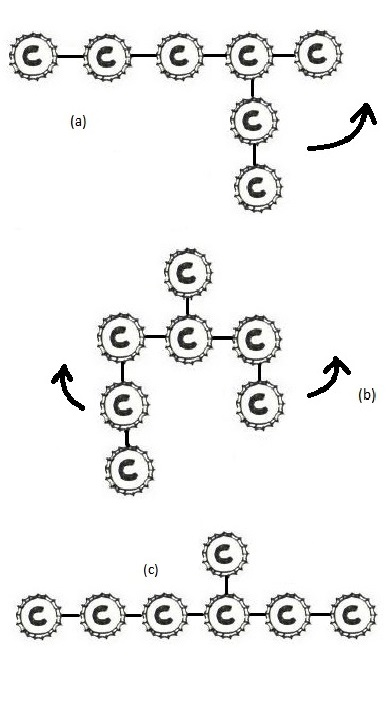
\includegraphics[width=0.45\textwidth]{./img/carbon-chain.jpg}
\end{center}

\begin{description*}
%\item[Subtopic:]{}
\item[Materials:]{Bottle caps, malleable wire (e.g. copper wire), tape}
\item[Setup:]{Tape bottle caps to a strip of wire as shown in a or b (at least 3 in a single line).}
\item[Procedure:]{Have students find and count the longest chain of bottle caps (carbon atoms) and write the name of the compound. Then bend the wire to show the actual longest chain (parent chain).}
%\item[Hazards:]{}
%\item[Questions:]{}
\item[Observations:]{Many students assume that any horizontal chain (a or b) is the parent chain. This is not always the case. Images a, b, and c are the exact same organic molecule, but c shows the correct parent chain has 6 carbons.}
\item[Theory:]{The parent chain of hydrocarbons is determined by counting the longest continuous chain of carbons. This is the arrangement in which the locant (or sum of locants) is lowest. Students often forget that the parent chain is not always in a straight line.}
%\item[Applications:]{}
%\item[Notes:]{}
\end{description*}

\vfill
\columnbreak

\subsection{Candles as Hydrocarbons}

\begin{center}
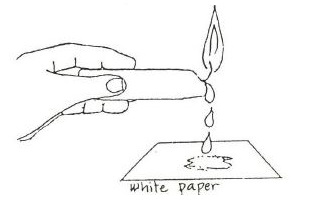
\includegraphics[width=0.4\textwidth]{./img/source/candle-hydrocarbon.jpg}
\end{center}

\begin{description*}
%\item[Subtopic:]{}
\item[Materials:]{Candle, paper}
%\item[Setup:]{}
\item[Procedure:]{Drop some liquid candle wax on a clean
white piece of paper.}
%\item[Hazards:]{}
\item[Questions:]{What happens to the paper? Why?}
\item[Observations:]{Candle wax produces a greasy not on paper.}
\item[Theory:]{Candle wax is chemically related to grease
fats and oils, it consists of long chain
hydrocarbons.}
%\item[Applications:]{}
%\item[Notes:]{}
\end{description*}

%==================================================================================================%

\section*{Alcohols}


\subsection{Preparation of Ethanol by Fermentation of Sugar}

%\begin{center}
%\includegraphics[width=0.4\textwidth]{./img/.png}
%\end{center}

\begin{description*}
%\item[Subtopic:]{}
\item[Materials:]{Gas generator, spatula, yeast, sugar, lime water, test tube}
%\item[Setup:]{}
\item[Procedure:]{Put 10-20 mL of lime water in a test tube and put the open end of the delivery tube from the gas generator into this solution. Make a sugar solution (3 spoonfuls sugar, 100 mL water). Add about 1~$^1$/$_2$ teaspoons of yeast and seal the bottle. Label the container and set it aside, checking daily for changes in the lime water.}
%\item[Hazards:]{}
%\item[Questions:]{What is the role of yeast in this experiment? What happens to the lime water in this experiment and what does this indicate?}
\item[Observations:]{When yeast is added to the sugar solution and left for some time, carbon dioxide is generated, which turns the lime water cloudy. The solution remaining in the bottle will have a faint smell of alcohol which shows the presence of ethanol.}
\item[Theory:]{Ethanol may be produced directly from petroleum, but for human consumption it is prepared by the fermentation of carbohydrates. Fermentation is the chemical breakdown of a substance by bacteria, yeasts, or other micro-organisms. Yeast breaks down sugar into alcohol and carbon dioxide gas.}
\item[Applications:]{Fermentation of starch or sugar produces many common alcoholic beverages, e.g. beer and wines.}
%\item[Notes:]{}
\end{description*}

\vfill
\columnbreak

\subsection[Reaction of Ethanol with Oxygen]{Reaction of Ethanol \hfill \\ with Oxygen}

%\begin{center}
%\includegraphics[width=0.4\textwidth]{./img/.png}
%\end{center}

\begin{description*}
%\item[Subtopic:]{}
\item[Materials:]{Colourless spirit, match box, soda cap with plastic removed, knife}
%\item[Setup:]{}
\item[Procedure:]{Put approximately 1 mL of ethanol into a soda cap. Light a match and touch it to the ethanol.}
\item[Hazards:]{Ethanol is flammable and the flame is hot. This activity should not be done on or around plastic or cloth material. Advise students that the flame may be colourless, thus special care must be taken. An ethanol flame can be extinguished with water if needed.}
\item[Questions:]{What happens when alcohol is lit with a match? What is the balanced chemical equation for the combustion of ethanol?}
\item[Observations:]{When the lit match is brought to the flame the ethanol burns in the presence of oxygen. A colourless flame will form.}
\item[Theory:]{One property of alcohols is that they readily combust. Ethanol burns readily in air with an almost colourless flame, producing carbon dioxide and water. The balanced chemical equation for this reaction is:\\

\ce{C2H5OH_{(l)} + 3O2_{(g)} $\longrightarrow$ 3H2O_{(g)} + 2CO2_{(g)}}}
%\item[Applications:]{}
%\item[Notes:]{}
\end{description*}

\vfill
\columnbreak

%==================================================================================================%

\section*{Carboxylic Acids}


\subsection{Reaction of Alcohol and Carboxylic Acid}

%\begin{center}
%\includegraphics[width=0.4\textwidth]{./img/.png}
%\end{center}

\begin{description*}
%\item[Subtopic:]{}
\item[Materials:]{Citric acid powder, methylated spirits, battery acid (5 M sulphuric acid), 2 beakers, tea spoon}
\item[Setup:]{Make a saturated solution of citric acid by mixing citric acid powder and clean water in a water bottle and shaking it until powder is dissolved.}
\item[Procedure:]{Put citric acid solution into one of the beakers. Take a small amount of the citric acid solution (about three water caps full) and pour it in the second beaker. Into the second beaker add about one cap full of battery acid and mix. To the mixture above add about three caps full of spirit and mix. Observe the smell.}
\item[Hazards:]{Battery acid is 5 M sulphuric acid. Concentrated sulphuric acid is corrosive to the skin and clothes. Avoid contact with skin and eyes. Neutralize spills with bicarbonate of sodium (baking soda).}
\item[Questions:]{Why was battery acid added to the citric acid solution? What smell did you detect in your experiment? Can you tell what the product is? What is the chemical reaction equation assuming that the spirit contains only ethanol?}
\item[Observations:]{Spirit reacts like ethanol and reacted with citric acid in the presence of acidic medium to produce a ester with fragrant smell.}
\item[Theory:]{One organic reaction of major importance is esterification. Esterification is the formation of an ester (ROOR') group through the reaction of an alcohol and a carboxylic acid. Many esters are volatile and their production can be observed by smell.}
%\item[Applications:]{}
%\item[Notes:]{}
\end{description*}


\end{multicols}

\pagebreak